\section{Kriterien-basierter Vergleich von Architektur Optionen}\label{sec:results:criteria}
\subsection{Einführung}
Dieses Kapitel vergleicht die Architektur-Alternativen anhand des Kriterienkatalogs. 

Die Schlussfolgerungen können aus der Beispielapplikation, aus der Theorie oder nicht gezogen werden. Aus diesem Grund habe ich die Schlussfolgerungen in verschiedene Güteklassen eingeteilt.

\begin{description}
    \item[Literatur] Die Werte des Vergleichs konnten aus der Literatur verweist werden.
    \item[Implementation] Die Werte des Vergleichs konnten durch die Beispielsapplikation gezeigt werden.
    \item[Theorie] Die Werte des Vergleichs konnten theoretisch durch eine Schlussfolgerung aufgezeigt werden.
    \item[Meinung] Die Werte entsprechen der Meinung des Architekten.
    \item[Nicht möglich] Der Vergleich konnte nicht gezeigt werden.
\end{description}

\subsection{Migrationsarbeit}

\paragraph{Ausarbeitungszeit des Konzeptes: Wie lange brauchte ich das Konzept auszuarbeiten?}

Diese Werte wurden durch die \textit{Implementation} bestimmt.

\begin{tabularx}{\linewidth}{| Y | Y | Y |}
    \hline
    Frontend-Komposition & Portal-Komposition & Backend-Komposition
    \\ \hline
    9 Stunden & 4 Stunden & 4 Stunden \\ \hline
\end{tabularx}

Bei der Frontend-Komposition sind viele Technologien notwendig gewesen um die Komposition aufzubauen. Ich hatte noch nicht mit diesen Technologien gearbeitet und musste mich in die Thematik einlesen. 

Der Kompositionsserver für die anderen Alternativen konnte mit Thymeleaf und WebClient\footnote{\url{https://docs.spring.io/spring-boot/docs/current/reference/html/boot-features-webclient.html}} aufgebaut werden.

\paragraph{Ausarbeitungszeit des Prototyps: Wie lange dauert die Ausarbeitung des ersten Prototyps der Architektur-Alternative?}

Diese Werte wurden durch die \textit{Implementation} bestimmt.

\begin{tabularx}{\linewidth}{| Y | Y | Y |}
    \hline
    Frontend-Komposition & Portal-Komposition & Backend-Komposition
    \\ \hline
    8 Stunden & 10 Stunden & 4 Stunden \\ \hline
\end{tabularx}

Die Portal-Komposition hat eine lange Entwicklungszeit, weil es schwierig war Thymeleaf zu konfiguriren, dass der Renderer die Fragmente von einem externen Service holt.

Die Frontend-Komposition hatte viele Technologien involviert mit welchen ich noch nicht gearbeitet hatte. Aus diesem Grund ist die produktivität geringer gewesen als bei der Backend-Komposition.

\paragraph{Fehler im Code: Wie viele Fehler hatte ich im Code?}

\begin{tabularx}{\linewidth}{| Y | Y | Y |}
    \hline
    Frontend-Komposition & Portal-Komposition & Backend-Komposition
    \\ \hline
    3 Fehler & 2 Fehler & 0 Fehler \\ \hline
\end{tabularx}

Die Frontend-Komposition hat sich als schwierige Technologie herausgestellt. Dank der Entscheidung Typescript\footnote{\url{https://www.typescriptlang.org/}} im Frontend einzusetzen konnten weitere, schwerwiegende Fehler frühzeitig erkannt werden.

Die Portal-Komposition hatte zweimal schwerwiegende Fehler, die wegen ungenauem Loggings der Thymeleaf Bibliothek schwierig zu erkennen waren.

\paragraph{Schrittweiser Übergang: Kann eine externe Seite im Micro-Frontend angezeigt werden?}

\begin{tabularx}{\linewidth}{| Y | Y | Y |}
    \hline
    Frontend-Komposition & Portal-Komposition & Backend-Komposition
    \\ \hline
    Ja (Literatur) & Ja (Implementation) & Nein (Implementation) \\ \hline
\end{tabularx}

Bei der Frontend-Komposition kann mit einem IFrame-Element kann eine externe Seite eingebunden werden.

Die Portal-Komposition kann mittels der Fragment-Auflösung von Thymeleaf externe Inhalte in die Page rendern.\cite{thymeleafURLtemplate}

Die Backend-Komposition nutzt den WebClient um die Daten beim Hintergrundservice abzurufen und rendert diese im Kompositionsserver mithilfe von lokalen Thymeleaf-Templates. Diese Technologie kann ohne das Zurückgreifen auf die Portal-Komposition keine Funktionsblöcke von der alten Website übernehmen.

\paragraph{Schrittweiser Übergang: Kann die alte Seite übernommen werden und im Aussehen auf die neue Seite angepasst werden?}

\begin{tabularx}{\linewidth}{| Y | Y | Y |}
    \hline
    Frontend-Komposition & Portal-Komposition & Backend-Komposition
    \\ \hline
    Nein (Literatur) & Ja (Implementation) & Nein (Implementation) \\ \hline
\end{tabularx}

Bei der Frontend-Komposition mit IFrames die Site nicht umgestaltet werden. \cite{mdnIFrame}

Es können Bereiche von anderen Websiten ausgespart werden und dann mit eigenen \ac{CSS} Regeln die Ansicht auf die neue Website angepasst werden.

Bei der Backend-Komposition kann das UI der alten Website nicht übernommen werden, da der Kompositionsserver kein \ac{HTML} verarbeitet.

\subsection{Aktualisierbar in Produktion}

\paragraph{Unterbrechungsfreie Aktualisierbarkeit: Kann das Microfrontend zusammen mit dem Microservice ausgetauscht werden?}

\begin{tabularx}{\linewidth}{| Y | Y | Y |}
    \hline
    Frontend-Komposition & Portal-Komposition & Backend-Komposition
    \\ \hline
    - (Nicht angesehen) & Ja (Implementation) & Nein (Implementation) \\ \hline
\end{tabularx}

Im Frontend wurde diese Fragestellung nicht weiter verfolgt um im Zeitplan zu bleiben. 

Bei der Portal-Integration muss nur der Applicationserver mit den UI-Fragmenten ausgetauscht werden.

Bei der Backend-Komposition liegen die Layout-Fragmente der Microfrontends auf dem Kompositionsserver, darum muss sowohl die Anwendungsserver als auch der Kompositionsserver ausgetauscht werden.

\subsection{Unabhängigkeit der Services}

\paragraph{Ausser der Abhängigkeit auf den Applikationserver darf das Frontend keine weitere Verbindungen benötigen.}

\begin{tabularx}{\linewidth}{| Y | Y | Y |}
    \hline
    Frontend-Komposition & Portal-Komposition & Backend-Komposition
    \\ \hline
    Ja (Implementation) & Ja (Implementation) & Ja (Implementation) 
    \\ \hline
\end{tabularx}

Alle Implementationen brauchen eine Abhängigkeit auf den Applikationserver um die Daten zu laden. Sie kommen mit dieser Abhängigkeit aus. 

\paragraph{Der Service darf keine Abhängigkeiten auf andere Services besitzen in der „Build-Phase“.}

\begin{tabularx}{\linewidth}{| Y | Y | Y |}
    \hline
    Frontend-Komposition & Portal-Komposition & Backend-Komposition
    \\ \hline
    Ja (Implementation) & Ja (Implementation) & Ja (Implementation) 
    \\ \hline
\end{tabularx}

Alle Alternativen haben keine Build-Dependency auf andere Services. 

Diese Forderung hängt von der verwendeten Kommunikationsbibliothek ab. Beispielsweise braucht WebClient keine Informationen über das Nachrichtenschema. Die Bibliothek WCF\footnote{\url{https://docs.microsoft.com/en-us/dotnet/framework/wcf/}} generiert zur Build-Zeit Code zum Verbindungsaufbau und braucht deshalb Informationen über das Message-Format des Kommunikationpartners.\cite{MicrosoftWCF}

Diese Forderung ist sehr Technologieabhängig, es kann jedoch ausgeschlossen werden, dass das Pattern eine solche Abhängigkeit verursacht.

\paragraph{Die Microfrontend Architektur darf nicht die Unabhängigkeit der Microservices erweichen}

\begin{tabularx}{\linewidth}{| Y | Y | Y |}
    \hline
    Frontend-Komposition & Portal-Komposition & Backend-Komposition
    \\ \hline
    Nein (Implementation) & Nein (Implementation) & Nein (Implementation) 
    \\ \hline
    Ja (Literatur) & Nein (Meinung) & Nein (Meinung)
    \\ \hline
\end{tabularx}

Die Implementation ist so geschrieben, dass die Frontend-Komponenten nicht in eigenen Projekten sind. Damit müssen alle Microfrontends ersetzt werden beim Deployment des Artefakts. 

Im Frontend könnte mit \citetitle{PolymerHomepage}\cite{PolymerHomepage} und \citetitle{mdnWebComponents}\cite{mdnWebComponents} die Trennung von Komponenten in einzelne Artefakte möglich sein. Dies wurde innerhalb dieser Arbeit nicht untersucht und könnte einen Ansatz für eine Folgearbeit bieten.

Aus technologischen Gründen unter Spring kann der Kompositionsserver nicht in verschiedene Files aufgetrennt werden. Aus diesem Grund sind die Frontend-Implementationen nicht unabhängige Prozesse und Komponenten. Es ist ein Server bei welchem alle UI-Ressourcen kompiliert werden und nicht austauschbar sind.

\paragraph{Services müssen einzeln aktualisierbar sein.}

\begin{tabularx}{\linewidth}{| Y | Y | Y |}
    \hline
    Frontend-Komposition & Portal-Komposition & Backend-Komposition
    \\ \hline
    Ja (Implementation) & Ja (Implementation) & Ja (Implementation) 
    \\ \hline
\end{tabularx}

Die Services haben in meiner Implementation keine Abhängigkeiten untereinander.

\subsection{Effekt auf die Geschwindigkeit}

\paragraph{Der Nutzer hat das Gefühl einer flüssigen Ladegeschwindigkeit}

\begin{tabularx}{\linewidth}{| Y | Y | Y |}
    \hline
    Frontend-Komposition & Portal-Komposition & Backend-Komposition
    \\ \hline
    Ja (Implementation) & Ja (Implementation) & Ja (Implementation)
    \\ \hline
\end{tabularx}

Alle Implementationen laden im Millisekundenbereich. Die Ladezeit der Frontend-Komposition ist leicht spürbar, da fast eine Sekunde. Nach dem Laden der \ac{UI} ist diese Variante die schnellste, da sie kein Backend-Rendering benötigt.

\paragraph{Die Ladegeschwindigkeit muss so schnell wie möglich sein.}

\paragraph{Die Zeit zur Auslieferung der Seite (\ac{TTFB}) muss so schnell wie möglich sein.}

\begin{tabularx}{\linewidth}{| Y | Y | Y |}
    \hline
    Frontend-Komposition & Portal-Komposition & Backend-Komposition
    \\ \hline
    Ja (Implementation) & Ja (Implementation) & Ja (Implementation) 
    \\ \hline
\end{tabularx}

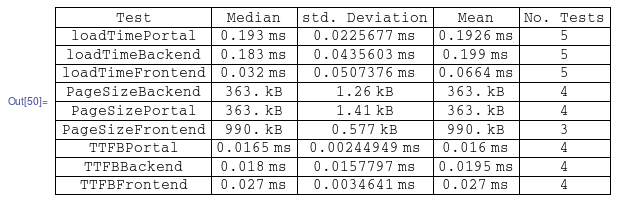
\includegraphics[width=\textwidth]{sections/results/PerformanceTests}

Die ersten drei Resultate beschreiben die gesamte Ladezeit einer Ansicht der Kompositionsvariante.

Die mittleren drei Resultate sind die Anzahl übertragener Bytes der Kompositionsvarianten.

Die untersten Datensätze beschreiben beschreiben die \ac{TTFB} der Varianten.

Wie aus der letzten Spalte zu entnehmen ist, ist in dieser SA eine sehr kleine Anzahl Tests verrichtet worden. Der Architekt geht davon aus, dass die Anzahl zu klein ist um genaue Aussagen über die Geschwindigkeiten zu treffen. Die Tabelle sollte für einen groben Überblick genommen werden, ist aber nicht als Feinvergleich der Implementierungen zu nehmen.

\paragraph{Die Zeit zwischen der Auslieferung und dem Fertigstellen des Renderings (Rendering Time) muss so schnell wie möglich sein.}

\begin{tabularx}{\linewidth}{| Y | Y | Y |}
    \hline
    Frontend-Komposition & Portal-Komposition & Backend-Komposition
    \\ \hline
    - (Nicht möglich) & - (Nicht möglich) & - (Nicht möglich) \\ \hline
\end{tabularx}

Ich konnte diesen Wert nicht messen, da in modernen Browsern das Rendering parallel zum Laden des Source-Codes ausgeführt wird. Wegen der Parallelität lässt sich nicht entscheiden, ob der Browser auf Daten gewartet hat oder der Renderer die Seite aufbaute.

\subsection{Theoretische Skalierbarkeit}

\paragraph{Die Kommunikation über das HTTP-Protokoll mit dem Applikationsserver muss stateless sein}

\begin{tabularx}{\linewidth}{| Y | Y | Y |}
    \hline
    Frontend-Komposition & Portal-Komposition & Backend-Komposition
    \\ \hline
    Ja (Implementation) & Ja (Implementation) & Ja (Implementation) \\ \hline
\end{tabularx}

In keinem Service wurde ein State eingeführt. Der Kompositionsserver ist ein Domain-spezifischer stateless Proxy.

\paragraph{Neue Instanzen können im Webserver Tier hochgefahren werden um die Anfragelast zu bewältigen.}

\begin{tabularx}{\linewidth}{| Y | Y | Y |}
    \hline
    Frontend-Komposition & Portal-Komposition & Backend-Komposition
    \\ \hline
    Ja (Implementation) & Ja (Implementation) & Ja (Implementation) 
    \\ \hline
\end{tabularx}

Weil die Kommunikation mit dem Browser stateless ist, ist dies zu jeder Zeit möglich.

\paragraph{Der Webserver darf keinen State, inklusive keine Session, des Nutzers speichern.}

\begin{tabularx}{\linewidth}{| Y | Y | Y |}
    \hline
    Frontend-Komposition & Portal-Komposition & Backend-Komposition
    \\ \hline
    Ja (Implementation) & Ja (Implementation) & Ja (Implementation) 
    \\ \hline
\end{tabularx}

Die Backend und Portal Integration sind stateless Proxies. Sie besitzen keine Informationen über vorherige Anfragen und müssen keine Annahmen über Anfragen in der Zukunft treffen können. Sie bekommen eine Anfrage und senden diese weiter an die Applikationsserver.

Der Webserver für die Frontend-Komposition ist stateless und liefert die HTML-Seite aus.

Die Frontend-Integration selber ist nicht stateless. Dies ist auf die Wahl des React-Frameworks zurück zu führen. Die Implementation muss die Daten nicht mehr anfragen, wenn diese bereits im Memory des Clients liegen. \cite{reactState}

\subsection{Informationssicherheit}

\paragraph{Die Vertraulichkeit (confidentiality) der Daten muss im Transport sichergestellt werden}

\begin{tabularx}{\linewidth}{| Y | Y | Y |}
    \hline
    Frontend-Komposition & Portal-Komposition & Backend-Komposition
    \\ \hline
    Ja (Meinung) & Ja (Meinung) & Ja (Meinung) 
    \\ \hline
\end{tabularx}

Durch \ac{TLS} kann die Verbindung zwischen Client und Server verschlüsselt werden. \cite{IetfTls} Dies wurde innerhalb des Projektrahmens nicht mehr realisiert. Aus diesem Grund, ist es die Meinung des Architekten, dass die Transportsicherheit bei allen Verfahren möglich ist. Der Architekt weist auf den Aufbruch der \ac{TLS}-Verbindung beim Kompositionsserver hin, dies kann ein Sicherheitsrisiko darstellen, da wegen dem Aufbruch der Verbindungen, auf diesem Server alle Verbindungen lesbar werden.

\paragraph{Die Integrität der Daten muss sichergestellt werden}

\begin{tabularx}{\linewidth}{| Y | Y | Y |}
    \hline
    Frontend-Komposition & Portal-Komposition & Backend-Komposition
    \\ \hline
    Ja (Implementation) & Ja (Implementation) & Ja (Implementation) \\ \hline
\end{tabularx}

Die Integrität der Daten kann einerseits sichergestellt werden durch Einsatz von Verschlüsselung zwischen den Services untereinander und dem Client. Wie bei der vorherigen Fragestellung erwähnt, können alle Alternativen adäquat verschlüsselt werden. 

\paragraph{Die Verfügbarkeit (availability) muss zu jeder Zeit sichergestellt sein}

\begin{tabularx}{\linewidth}{| Y | Y | Y |}
    \hline
    Frontend-Komposition & Portal-Komposition & Backend-Komposition
    \\ \hline
    Nein (Implementation) & Nein (Implementation) & Nein (Implementation) \\ \hline
\end{tabularx}

Keine Alternative garantiert die Verfügbarkeit der Daten. Die Frontend-Komposition hat den Vorteil, dass sie ohne einen Kompositionsserver auskommt und eine Komponente weniger hat, die nicht verfügbar sein kann.

\paragraph{Die Services dürfen keine Daten und keine Frontend-Fragmente ausliefern an unberechtigte, dritte Personen.}

\begin{tabularx}{\linewidth}{| Y | Y | Y |}
    \hline
    Frontend-Komposition & Portal-Komposition & Backend-Komposition
    \\ \hline
    Nicht untersucht (Implementation) & Nicht untersucht (Implementation) & Nicht untersucht (Implementation) \\ \hline
\end{tabularx}

Das \ac{AAA} wurde innerhalb dieser Arbeit nicht untersucht und kann als Fortsetzung dieser Arbeit aufgegriffen werden.